\section{Tree to Random Forest}
\subsection{Decision Tree}

\begin{frame}
	\frametitle{Decision Tree: Example}
	\begin{figure}		
		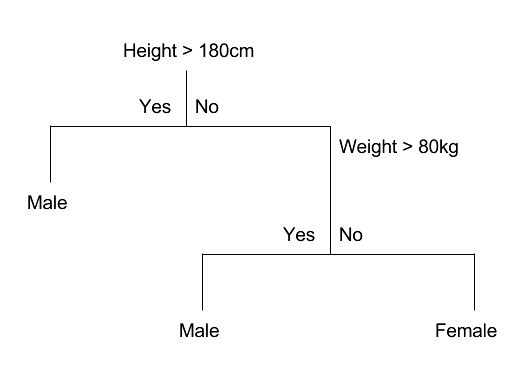
\includegraphics[height=0.7\textheight]{images/decision_tree_example.png}
		\caption{Source:\cite{james2013learning} }
	\end{figure}
\end{frame}

\begin{frame}
	\frametitle{Decision Tree: Tree Building Process}
	A tree is grown starting from the root node by repeatedly 
	using the following steps on each node (also called binary splitting) \cite{breiman1984classification}:
	\begin{enumerate}
		\item[(i)] \textbf{Find best split \(s\) for each feature \(X_{m}\):}
		For each feature \(X_{m}\), there exist \(K-1\)-many potiential splits whereas \(K\) is the number of different values for the respective feature.
		Evaluate each value \(X_{m,i}\) at the current node \(t\) as a candidate split point (for \(x \in X_{m}\), if \(x \leq X_{m,i}=s\),
		then \(x\) goes to left child node \(t_{L}\) else to right child node \(t_{R}\)).
		The best split point is the one that maximize the splitting criterion \(\ \Delta i(s,t) \) the most when the node is split according to it.
		The different splitting criteria will be covered in the next chapter.
		\item[(ii)] \textbf{Find the node’s best split:} Among the best splits for each feature from Step (i) find the one \(s^{*}\), which maximizes the splitting criterion \(\Delta i(s,t)\).
		\item[(iii)] \textbf{Satisfy stopping criterion:} Split the node \(t\) using best node split \(s^{*}\) from Step (ii) and 
		repeat from Step (i) until stopping criterion is satisfied. 
	\end{enumerate}
\end{frame}	

\begin{frame}
	\frametitle{Decision Tree: Purity Measures}
	\begin{block}{Gini Measure}
		\begin{equation}    
			i(t) = \sum_{c \in C} p(c|t) (1 - p(c|t)) = 1 - \sum_{c \in C} p_{c}^{2}
		\end{equation}
	\end{block}
	\begin{block}{Information Entropy}
		\begin{equation}    
			i(t) = \sum_{c \in C} p(c|t) log(p(c|t))
		\end{equation}
	\end{block}	
\end{frame}